% !TeX spellcheck = hu_HU
% !TeX encoding = UTF-8

\chapter{Infrastruktúramenedzsment: Uyuni}
Nagyméretű informatikai infrastruktúra kezelése esetén elengedhetetlen valamiféle infrastruktúramenedzsment-eszköz használata. Ez nem csak könnyebbé teszi az üzemeltetést, de számos kiegészítő funkcióval is rendelkezik, lényegében egy helyen láthatunk minden releváns adatot, és egyazon felületről van lehetőségünk frissítések telepítésére és biztonsági sérülékenységek leírásainak böngészésre, mint ahol azt is tároljuk, hogy egy adott virtuális gép melyik gazdagépen fut, és az hol található.

Mivel ez a megoldás hasznosnak és érdekesnek tűnt számomra, és a dolgozat profiljába is jól illeszkedik, úgy döntöttem, hogy a tesztkörnyezet kezelésére is fogok ilyen megoldást alkalmazni. A választásom az Uyuni-ra esett, mely gyakorlatilag mindent tud, amire szükségem volt, és ingyenesen elérhető. A döntésben az is segített, hogy a projektet a SUSE támogatja, a fejlesztésében is részt vesz (az Uyuni szolgál a kereskedelmi forgalomban lévő SUSE Manager megoldás alapjául), és az openSUSE-alapú disztribúciókra is kiemelt figyelmet fordítanak, így nem kellett kompatibilitási problémákkal foglalkoznom. Az Uyuni a Salt konfigurációmenedzsment és automatizációs keretrendszerre épül, mely szintén széleskörűen használt és támogatott.


\section{Telepítés}
\label{sect:uyuni-install}
Az Uyuni meglehetősen erőforrás-igényes, a telepítéséhez minimum négy CPU-mag, 16~GB memória és  több száz gigabyte tárhely lehet szükséges a használni kívánt telepítőforrásoktól függően~\cite{UyuniInstallGuide}. Éles környezetben még ennél is több memóriát javasolnak, így az Uyuni számára létrehozott virtuális gép lett a környezet leginkább erőforrás-igényes rendszere, melynek telepítéshez használt parancs és a \acrshort{vm} leírója látható \aref{lst:virtinstall} és \aref{lst:virshxml} kódrészleteken. Ezeken megfigyelhetjük, hogy a virtuális gépet 12~CPU-maggal és 32~GB memóriával hoztam létre, a particionálásra a későbbiek folyamán fogok részletesen kitérni.

Ahogy a korábbiakban írtam, az Uyuni jó támogatottságnak örvend az openSUSE platformon. A telepítési kézikönyvben egy dedikált openSUSE Leap 15.5-ös \acrshort{os}-verziót futtató számítógépet javasolnak az infrastruktúramenedzsment-program telepítéséhez~\cite{UyuniInstallGuide}.
Ennek megfelelően én is ezt a verziót telepítettem, és bár a Leap alapértelmezett telepítési forrásaiban nem szerepel az Uyuni, de az ezt tartalmazó telepítőforrást egyetlen paranccsal felvehetjük, és ezt követően a segítségével telepíthetjük is az Uyunit.

\subsection{Kötetkiosztás}
A particionálás kérdése azért is kiemelt fontosságú az Uyuni telepítése során, mert a telepítés folyamán ezen feltételek meglétét ellenőrzi is a telepítő, és nem teljesülésük esetén a telepítés hibára futhat. A kötetek kiosztása során a hivatalos útmutatóból indultam ki, viszont a felhasználási célok figyelembevételével néhány partíciót a javasoltnál nagyobbra állítottam be, ennek megfelelően jött létre \aref{tab:uyuni-partitioning}.~táblázatban ismertetett felépítés. Elsősorban a spacewalk kötet növelése volt indokolt, hiszen az Uyuni egyik fontos része a szoftvercsomagok kezelése. Ennek gördülékeny és hatékony használatához a rendszer letükrözi a szükséges telepítőforrásokat, melyek jelentős helyigénnyel rendelkeznek, melyre \aref{sect:reposync} alfejezetben térek ki részletesen.

\begin{table}[h]
	\setlength{\tabcolsep}{5pt}
	\renewcommand{\arraystretch}{1.3}
	\centering
	\begin{tabular}{||l l l l m{5.3cm}||}
		\hline
		Kötet & Csatolási pont & Méret & Típus & Leírás\\
		\hline\hline
		boot & /boot & 1~GB & fizikai, ext4 & Az \acrshort{os} betöltéséhez szükséges fájlok tárhelye. \\
		\hline
		root & / & 40~GB & \acrshort{lvm}, XFS & A könyvtár-hierarchia legfelső eleme, a rendszerfájlok helye. \\
		\hline
		pgsql & /var/lib/pgsql & 52~GB & \acrshort{lvm}, XFS & A PostgreSQL adatbázismotor által tárolt adatok könyvtára. \\
		\hline
		spacewalk & /var/spacewalk & 100~GB & \acrshort{lvm}, XFS & Az infrastruktúramenedzsment\Hyphdash szoftver által használt fájlok elsődleges helye. \\
		\hline
		cache & /var/cache & 12~GB & \acrshort{lvm}, XFS & Gyorsítótárazott adatok könyvtára. \\
		\hline
		swap & swap & 4~GB & \acrshort{lvm}, swap & Virtuális memóriaként használt lemezterület. \\
		\hline
	\end{tabular}
	\caption{Az infrastruktúramenedzsment-szerver telepítéskori kötetkiosztása.}
	\label{tab:uyuni-partitioning}
\end{table}

\section{Telepítőforrások tükrözése}
\label{sect:reposync}
Ahogy az előző alfejezetben már említettem, az Uyuni egyik központi feladata a telepítőforrások és szoftvercsomagok kezelése a bevont rendszereken. Ehhez a használni kívánt telepítőforrásokat le kell tükröznünk az Uyunit futtató szerverre. Ez a megoldás elsőre túlzásnak tűnhet, hiszen egy-egy ilyen forrás több tíz, egyes esetekben több száz gigabyte lehet, azonban egy nagyméretű infrastruktúránál megvannak az előnyei. Gondoljunk csak bele, hogy mekkora hálózati forgalmat takaríthatunk meg azzal, hogy a telepítendő szoftverek és operációsrendszer-frissítések letöltésekor nem kell minden esetben az internetről letölteni a szükséges csomagokat, hanem ezt elegendő mindössze egyszer, az Uyuni szerveren megtenni, és onnantól kezdve az összes kliens már a belső hálózatról érheti el a szükséges programokat.
Emellett hasznos lehet egy offline példány megtartása is a telepített csomagokból, hiszen előfordulhat, hogy egy harmadik fél által üzemeltetett telepítési forrás elérhetetlenné válik, és így nem férünk hozzá a kívánt csomagokhoz.

Ahhoz, hogy egy-egy ilyen csomagtárhelyet letükrözhessünk, létre kell hozni úgynevezett \textit{Software Channel}-eket, melyek lényegében a repository-t csomagolják be egy magasabb szintű egységbe. Ez tárolja, hogy milyen csomagok érhetőek el, ezek milyen architektúrán használhatóak, lehetővé teszik a csomagforrások kezelését, és hozzárendelhetjük őket a kliensekhez. A csatornák által tartalmazott repository-k tárolják, hogy milyen címen érhető el a tükrözendő telepítőforrás, és hogy az adott repository melyik csatornához van hozzárendelve.

A tesztkörnyezethez is tükröztem telepítési forrásokat. Mivel a gépek többsége openSUSE Leap~15.5-ös verziót használt, ezért az ehhez tartozó csomagok szinkronizálásával kezdtem. Minden alapértelmezett forrást letükröztem, illetve az Uyuni általi menedzselés céljából az Uyuni-csomagokat tartalmazó repository-t is felvettem a szinkronizálandók közé. Az egyszerűbb kezelés miatt a csatornák hierarchiába szervezhetőek, így csak a kiválasztott szülőcsatornával (base channel) kompatibilis gyermekcsatornákat vehetünk fel egy adott klienshez. A tesztkörnyezetben létrehozott telepítőforrás-hierarchiát \aref{fig:software-channels}.~ábra szemlélteti.

\begin{figure}[ht]
	\centering
	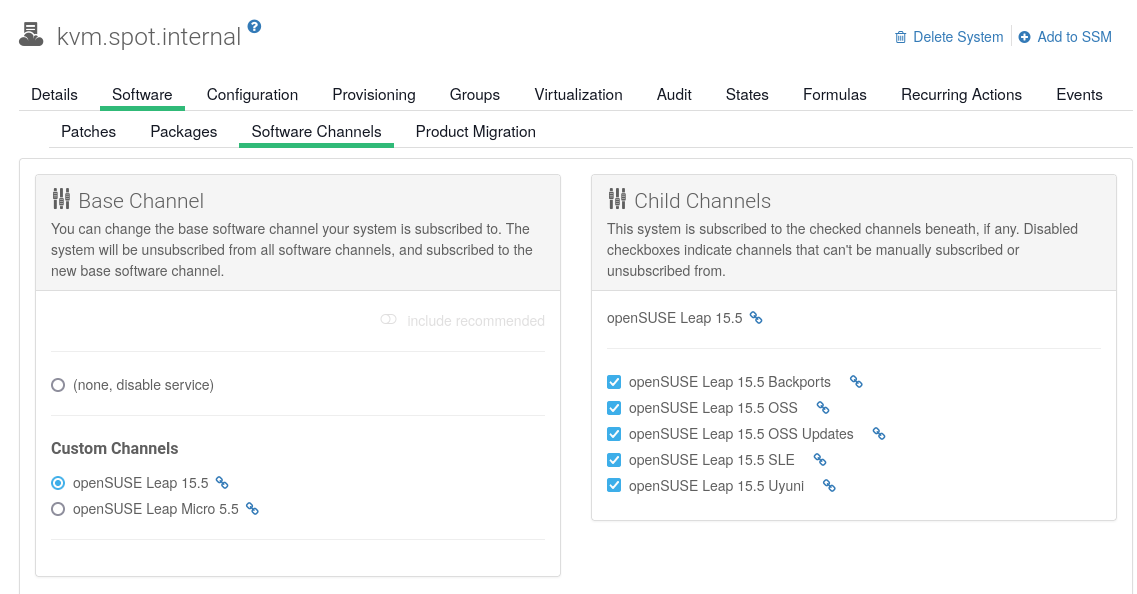
\includegraphics[width=15cm]{figures/uyuni-channels.png}
	\caption{A kialakított csatornahierarchia.}
	\label{fig:software-channels}
\end{figure}

Az első repository tükrözése a vártnál közel 20\%-kal több tárhelyet igényelt a spacewalk köteten (\ref{fig:reposync-disk-usage}.~ábra), így szükségessé vált a partíció megnövelése. Ennek megvalósításához az~\acrshort{lvm} által biztosított \texttt{lvextend} parancsot használtam, mely a logikai kötet megnövelésén túl a fájlrendszer (itt XFS) kiterjesztését is támogatja. Ez a parancs viszont csak akkor használható, ha a kötetcsoportban~(\acrshort{vg}) rendelkezésre áll annyi szabad hely, amennyivel bővíteni szeretnénk a tárhelyet. Mivel azonban itt ez a feltétel nem teljesült, több szinten kellett elvégezni a kötet megnövelését, először a~\acrshort{kvm}-hoszton kellett megnövelni a virtuális géphez tartozó tárterületet. További kihívást jelentett, hogy a kiterjesztést a~\acrshort{vm} leállítása nélkül szerettem volna elvégezni. Ebben az esetben nem jelentett volna nagy gondot a gép újraindítása, viszont szerettem volna felkészülni olyan helyzetekre is, amikor a gép leállítása nem megengedhető. Ilyen lehet például, ha a szinkronizálás alatt álló telepítőforrás a vártnál jelentősen nagyobb méretűnek bizonyul, vagy éppen a~PostgreSQL által használt tárhely van fogytán, de még nem fejeződött be a korábban indított indexelés. Mindezek mellett általában éles környezetben is korlátozottak a lehetőségeink egy-egy kiszolgáló újraindítására.

\begin{figure}[ht]
	\centering
	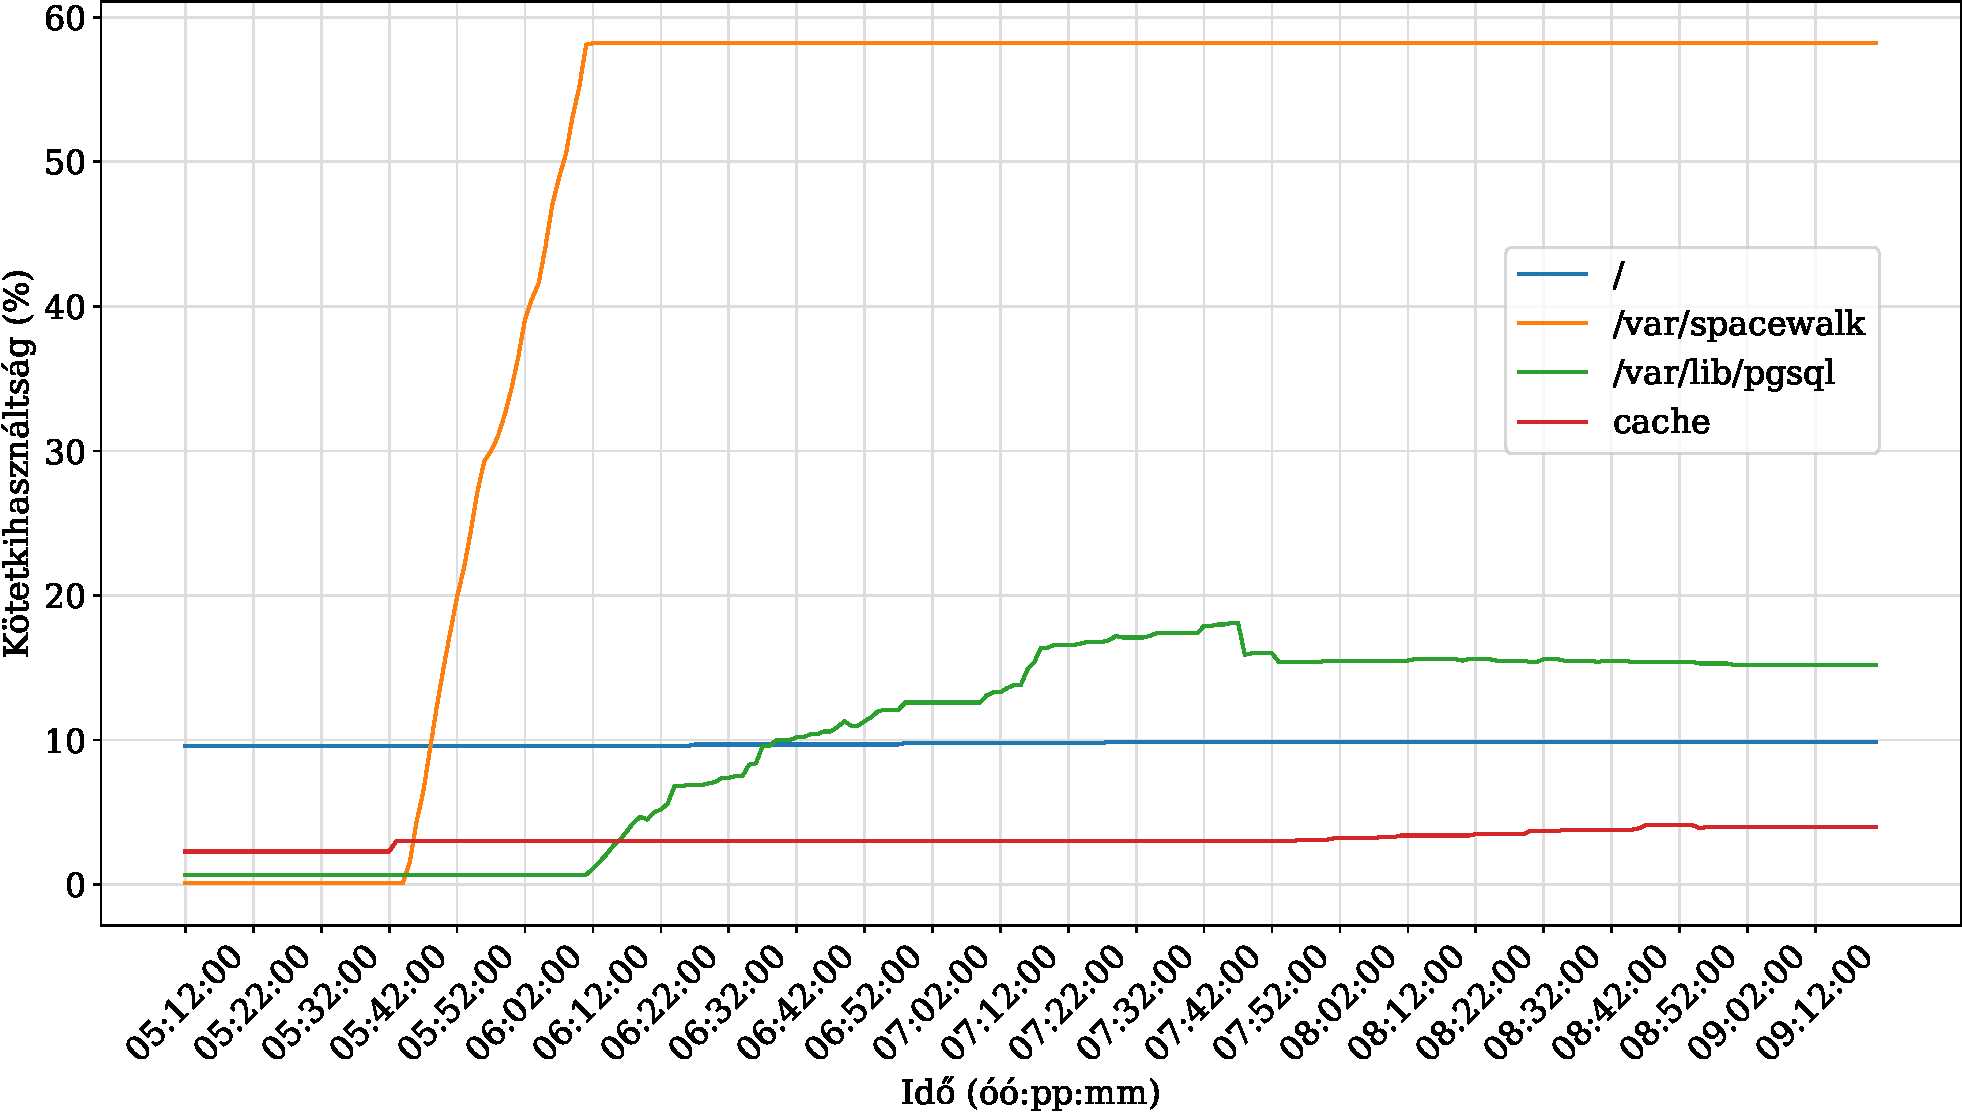
\includegraphics[width=15cm]{figures/reposync-leap-oss-disk-grid.pdf}
	\caption{Kötetkihasználtság változása az egyik telepítőforrás tükrözése során.}
	\label{fig:reposync-disk-usage}
\end{figure}

\subsection{Online kötetnövelés}
Ezen okokból a spacewalk kötet online megnövelése mellett döntöttem. Első lépésként a hosztgépen terjesztettem ki a virtuális gép számára fenntartott partíciót (a~\texttt{kvm-uyuni} logikai kötetet). \Aref{lst:virsh-blockresize}. kódrészleten látható, hogy ezt követően a virtuális gép még nem tudja használni a nagyobb méretű kötetet, szükséges még a \texttt{virsh blockresize} parancs futtatása, melynek hatására a virtuális gép számára is láthatóvá válik a nagyobb kötetméret. Ezt követően a~\acrshort{vm}-en növeltem meg a logikai kötetek alapjául szolgáló fizikai kötet~(\acrshort{pv}) méretét, melyet követően már a megszokott módon volt lehetőség a logikai kötet bővítésére.

\begin{lstlisting}[caption=Az infrastruktúramenedzsment-programokat futtató virtuális gép kötetének online megnövelése a gazdagépen.,label=lst:virsh-blockresize,escapechar=?]
	?\underline{10-151-7-5:$\sim$ \#}? virsh domblkinfo uyuni /dev/vg1/kvm-uyuni
	Capacity:       268435456000
	Allocation:     225145827328
	Physical:       375809638400
	?\underline{10-151-7-5:$\sim$ \#}? virsh blockresize uyuni --path /dev/vg1/kvm-uyuni --size 350G
	Block device '/dev/vg1/kvm-uyuni' is resized
	?\underline{10-151-7-5:$\sim$ \#}? virsh domblkinfo uyuni /dev/vg1/kvm-uyuni
	Capacity:       375809638400
	Allocation:     225145827328
	Physical:       375809638400
\end{lstlisting}

\section{Kliensek felvétele}
A kliensek felvétele során mutatkozott meg az Uyuni egy kisebb hátránya az előfizetés-alapú SUSE~Manager-rel szemben. Míg az előfizetésért cserébe előre konfigurált csatornákat (ún. Product-okat) kapunk, addig az Uyunihoz ez nem áll rendelkezésünkre, a kliensek felvételéhez használt bootstrap megoldás pedig csak ezekkel működik együtt. A bootstrap folyamat sikeres futtatása többszörös próbálkozást követően sem sikerült~(\ref{fig:uyuni-bootstrap-error}. ábra). Emiatt az elsődleges konfiguráció során manuálisan kellett gondoskodnom a szükséges csomagok telepítéséről és az ezekhez kapcsolódó beállítások elvégzéséről. A gyakorlatban ez azt jelentette, hogy a kezelni kívánt rendszerekre telepíteni kellett a \texttt{venv-salt-minion} csomagot, emellett szükséges volt két konfigurációs fájl létrehozása is, melyek a Salt minion azonosítóját (amilyen néven a gép megjelenik az~Uyuni felületén) és a Salt master (az~Uyuni szerver) IP-címét tartalmazták~(\ref{lst:salt-client-config}.~kódrészlet).
Ezt követően a kapcsolódó Salt service újraindításával a kliens kapcsolatot kezdeményezett a Salt masterrel, és az Uyuni felületén lehetővé vált a kliens csatlakozási kérelmének elfogadása. A kérelem elfogadását követően az Uyuni lekérdezett néhány adatot a kliens állapotáról (pl. telepített csomagok, hardveres erőforrások), ez után az újonnan bevont rendszer már teljes körűen kezelhetővé vált az Uyuni felületén keresztül.

\begin{figure}[ht]
	\centering
	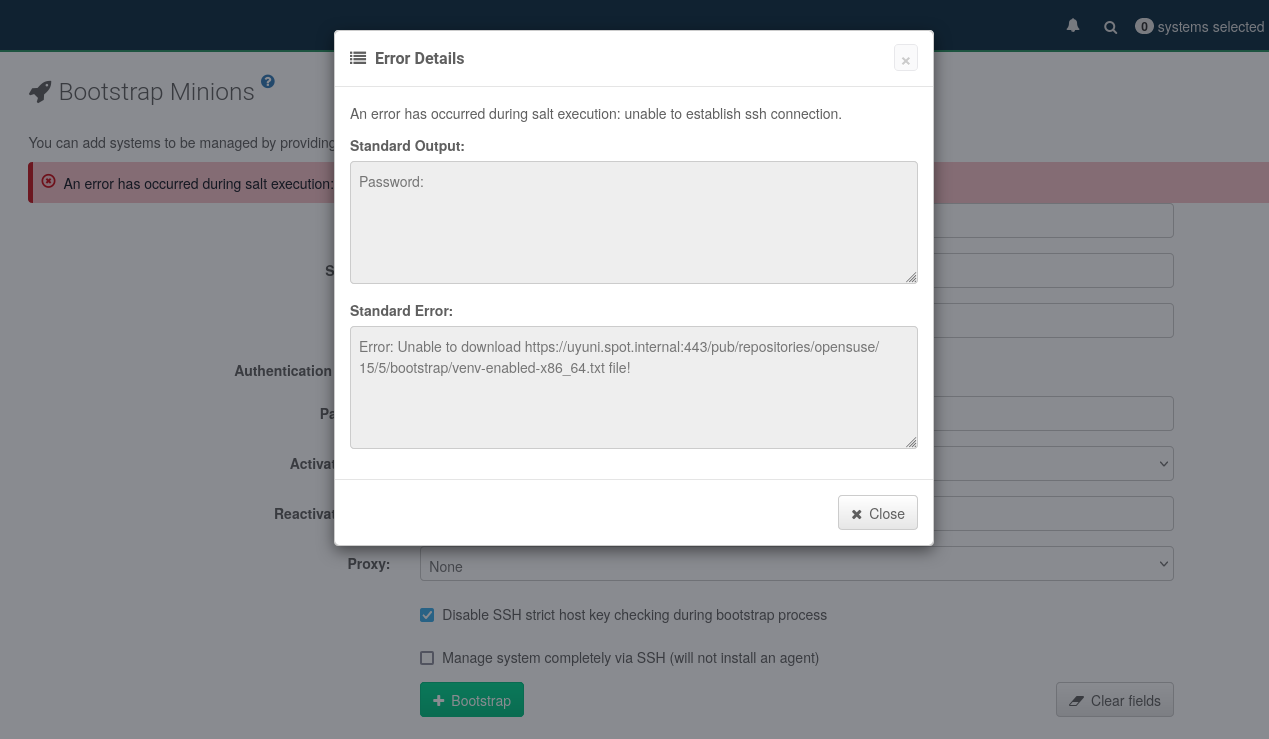
\includegraphics[width=15cm]{figures/uyuni-bootstrap-error.png}
	\caption{Előfizetés nélkül nem érhetőek el a product repository-k.}
	\label{fig:uyuni-bootstrap-error}
\end{figure}


\begin{figure}[ht]
	\centering
	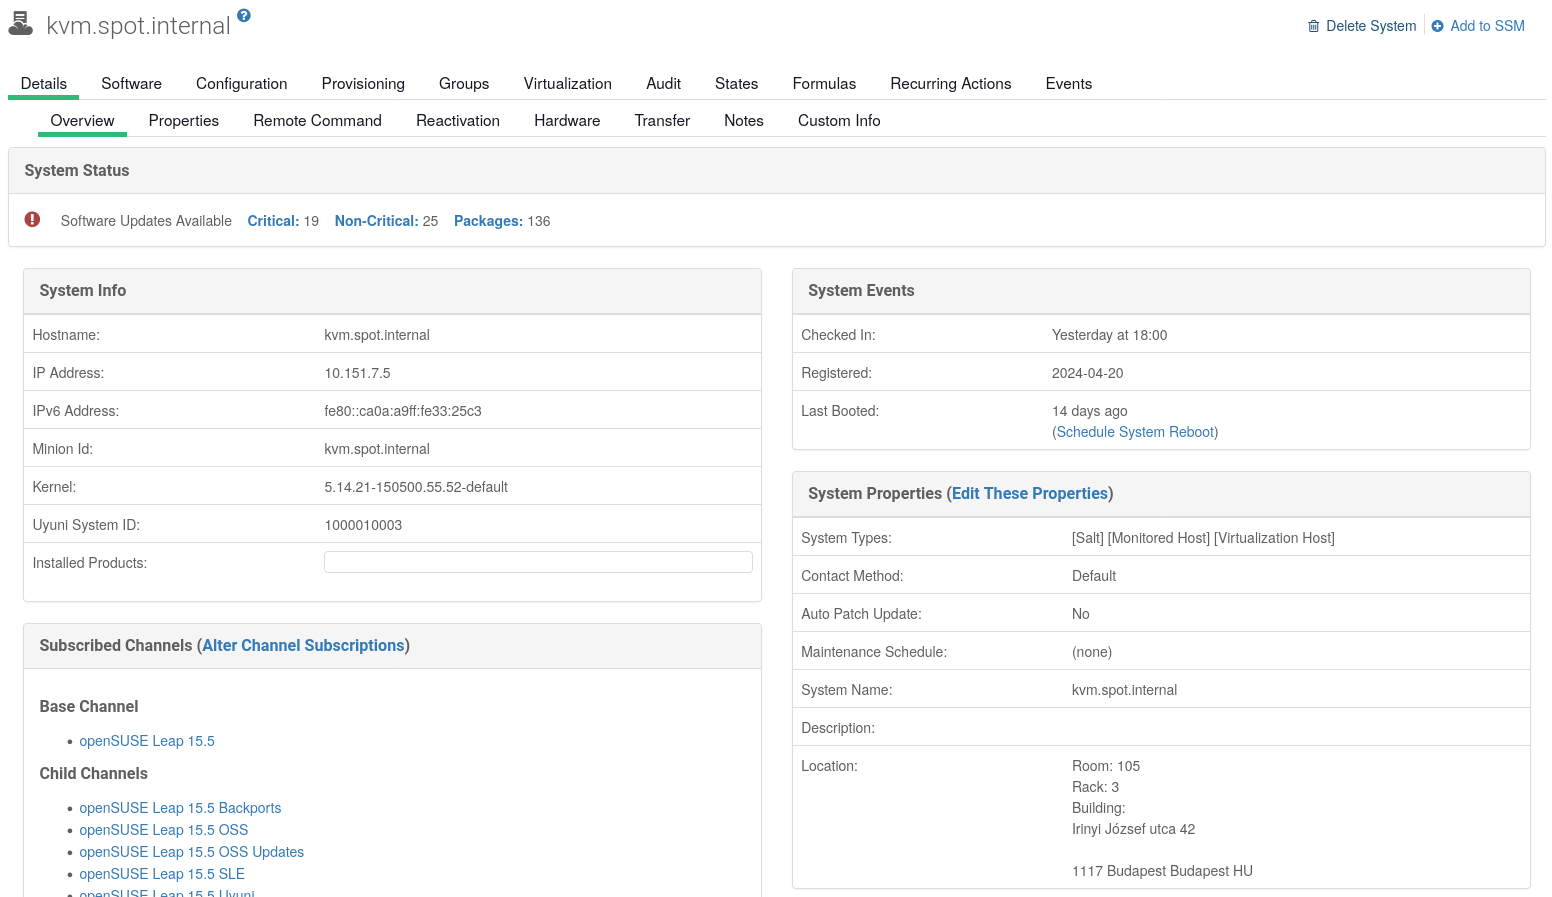
\includegraphics[width=15cm]{figures/uyuni-system-details.png}
	\caption{A bevont rendszer adatainak frissítését követően számos részletet láthatunk a gépről, és mi is adhatunk meg bizonyos adatokat.}
	\label{fig:uyuni-system-details}
\end{figure}

\begin{lstlisting}[caption=A manuális konfiguráció során létrehozott állományok.,label=lst:salt-client-config,escapechar=?]
	?\underline{10-151-7-5:/etc/venv-salt-minion/minion.d \#}? cat id.conf
	id: kvm.spot.internal
	?\underline{10-151-7-5:/etc/venv-salt-minion/minion.d \#}? cat master.conf
	master: 10.151.7.1
\end{lstlisting}

\subsection{Rendszertípusok és Salt Formulák}
A kezdeti információgyűjtés során az infrastruktúramenedzsment-rendszer megpróbálja meghatározni a rendszer típusát (fizikai gép, virtualizációs gazdagép, virtuális gép). Ezeket később mi is megadhatjuk, illetve a betöltött szereptől függően úgynevezett Salt Formulákat rendelhetünk hozzájuk. Ezek olyan előre elkészített Salt state fájlok, melyek a gyakran használt beállítások megadását igyekszenek egyszerűbbé tenni.

Munkám során én két rendszertípust használtam: a virtualizációs hoszthoz és a monitorozott rendszerhez kapcsolódót. A \textit{Virtualization Host} Formula néhány alapvető beállítást (pl. hálózati konfiguráció) ad meg a rendszeren, azonban ez a felhasználási céljaimnak nem felelt meg teljes mértékben, így a beállításokat egy saját Salt state-tel módosítottam, mely a~\ref{lst:vhost-salt-formula-mod}~kódrészleten látható. A példában a könnyebb átláthatóság érdekében a módosítandó fájl tartalmát a state fájlban definiáltam, de lehetőség van ennek egy központilag, az Uyunin keresztül kezelt konfigurációs fájl hivatkozásával való megadására is.
A \textit{Monitored Host} beállításait a következő fejezetben tárgyalom részletesen.

\begin{lstlisting}[caption=A hálózati konfiguráció frissítését végző Salt state.,label=lst:vhost-salt-formula-mod]
update_/etc/sysconfig/network/ifcfg-br0:
	file.managed:
		- name: /etc/sysconfig/network/ifcfg-br0
		- user: root
		- group: root
		- mode: 644
		- content: |
			BOOTPROTO='dhcp'
			STARTMODE='onboot'
			ZONE='public'
			BRIDGE='yes'
			BRIDGE_PORTS='eth1'
			BRIDGE_STP='off'
\end{lstlisting}

\section{Szolgáltatások telepítése, kezelése}
Az Uyuni egy fontos része a konfiguráció-menedzsment és a szoftvercsomagok telepítése, frissítése. Ezekre elsősorban Salt state-eken keresztül nyújt támogatást, a tesztkörnyezetben én is a Salt-alapú megoldást választottam a csomagok telepítésére.

Csomagok és azok konfigurációjának kezeléséhez létre kell hoznunk egy konfigurációs csatornát, egy úgynevezett state channelt, mely tartalmazni fogja az elkészített state fájlt és az esetlegesen használt konfigurációs állományokat. A state fájl megírását követően a csatorna hozzárendelhető a kezelt hosztokhoz.

Miután ez megtörtént, a gépekre, melyekhez hozzárendeltük az adott state-et, ki kell küldeni egy úgynevezett highstate-et. Ez egy különleges state, melyet a rendszer állít elő a feliratkozott state-ek tartalmából, a feliratkozási hierarchiát figyelembe véve. A highstate tehát minden hozzárendelt state channel adatait  tartalmazza, és a lefuttatásával jutnak érvényre a frissen felvett módosítások is. \Aref{fig:uyuni-channelsub}.~ábrán látható, hogy az Uyuni lehetőséget biztosít több kliens kiválasztására is, ezt kihasználva két hosztra egyszerre alkalmaztam a módosításokat.

\begin{figure}[ht]
	\centering
	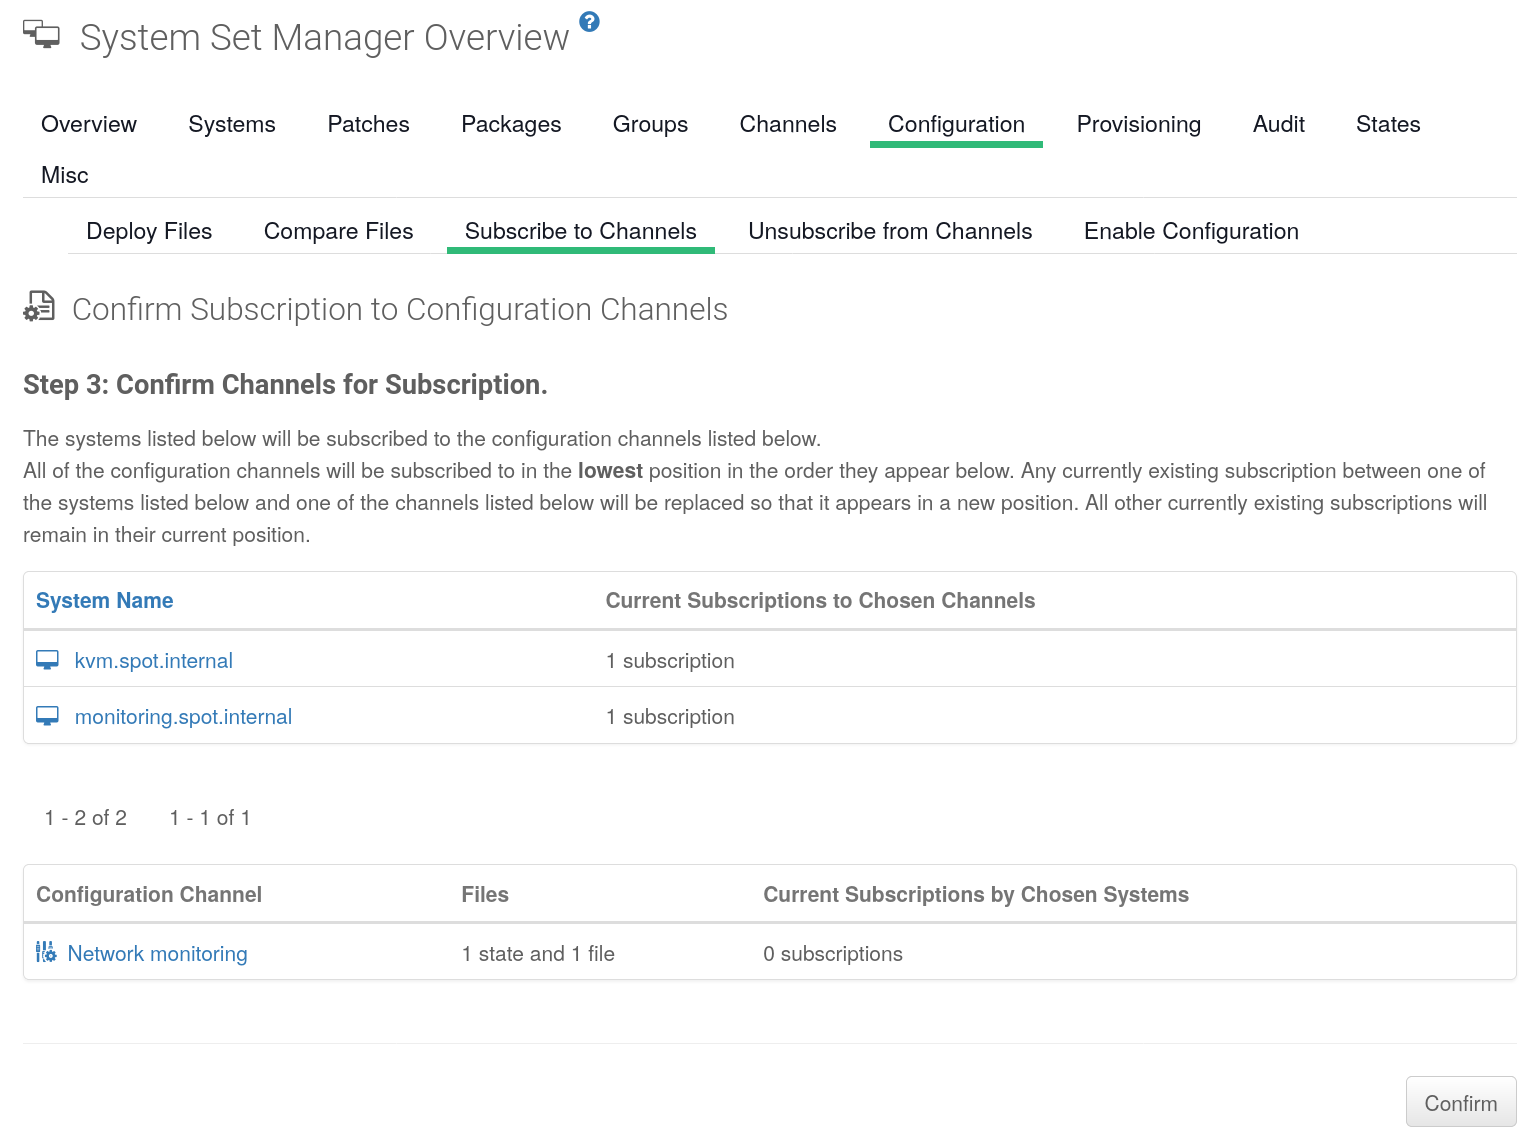
\includegraphics[width=15cm]{figures/uyuni-channelsub.png}
	\caption{Két kiszolgáló feliratkoztatása a \textit{Network monitoring} state channelre.}
	\label{fig:uyuni-channelsub}
\end{figure}

A fenti példában használt channel state fájlja \aref{lst:network-monitoring-state}.~kódrészleten látható. Ezzel néhány, a hálózati forgalom monitorozását lehetővé tevő csomagot telepítettem a feliratkozott gépekre, illetve elindítottam a kapcsolódó service-t és felülírtam az alapértelmezett konfigurációs állományt egy némileg különbözővel, ami alapértelmezetten más mértékegységeket használ a forgalom monitorozása során.

A state konfigurálásához éltem a Salt által nyújtott sablonozási lehetőséggel, mely lehetőséget biztosít például változók létrehozására, \texttt{if-else}~ágak meghatározására, és \texttt{for}~ciklus használatára is. Bár ez elsőre némi többletmunkát jelent a state létrehozása során, egy sokkal karbantarthatóbb megoldást eredményez, hiszen elegendő például a telepítendő csomagokat egy listában felsorolni, melyet bármikor bővíthetünk, és nem kell egy-egy csomópontot lemásolni újabb hibalehetőségek esetleges bevezetésével. A sablonozás további előnye, hogy futásidőben is lekérdezhetjük például egy fájl létezését, és ez alapján folytathatjuk a state végrehajtását. Ilyen megoldást szemléltet a state forráskódjának 10.~sora, melyben az elágazás megvizsgálja, hogy éppen telepítésre kerül-e a \texttt{vnstat} csomag, vagy ha nem, akkor egy létező konfigurációs állományt szeretnénk-e frissíteni. Az elágazás eredménye függvényében frissíti a fájlt, vagy változatlanul hagyja. Egy másik hatékony megoldás az úgynevezett \textit{grain}-ek használata, melyek lehetővé teszik részletes információk lekérdezését egy Salt kliensről. Ilyet használtam a forráskód 21.~sorában, ahol az~\acrshort{os}-család függvényében más-más néven tudtam elérni a vnstat háttérfolyamatát.

\lstinputlisting[caption=A Network monitoring konfigurációs csatornához tartozó Salt state.,label=lst:network-monitoring-state, numbers=left]{listings/netmonitoring-init.sls}

\section{Erőforrásigény mérése}
A fejezet elején ismertetett komoly erőforrásigény miatt kíváncsi voltam a hardver adta lehetőségek tényleges kihasználtságára. Mivel ekkor még nem állítottam be a monitoring rendszert~(ehhez előbb be kellett fejeznem az Uyuni konfigurációját), ezért egy saját Python scriptet készítettem az erőforrások állapotának figyelésére.

A mérést egy telepítőforrás-tükrözés során végeztem, hiszen ekkor volt a legnagyobb a rendszer erőforrásigénye. A jelentős mértékű hálózati adatforgalmat követően -- melyet a szoftvercsomagok letöltése idéz elő -- a rendszer hosszas adatbázis-indexelést hajt végre, mely során a processzormagok kihasználtsága közel 100\%-os. A mérési adatokból készített grafikon~\aref{fig:reposync-chart}.~ábrán látható. Jól megfigyelhető, hogy a kezdeti nagy hálózati forgalommal párhuzamosan a spacewalk kötet kihasználtsága is gyorsan nő. A letöltés befejeztével megkezdődik az adatbázis-indexelés, mely során a számítási kapacitás kihasználtságának növekedése tapasztalható, emellett pedig a várakozásoknak megfelelően az adatbázisköteten nő a foglalt terület.


\begin{figure}[ht]
	\centering
	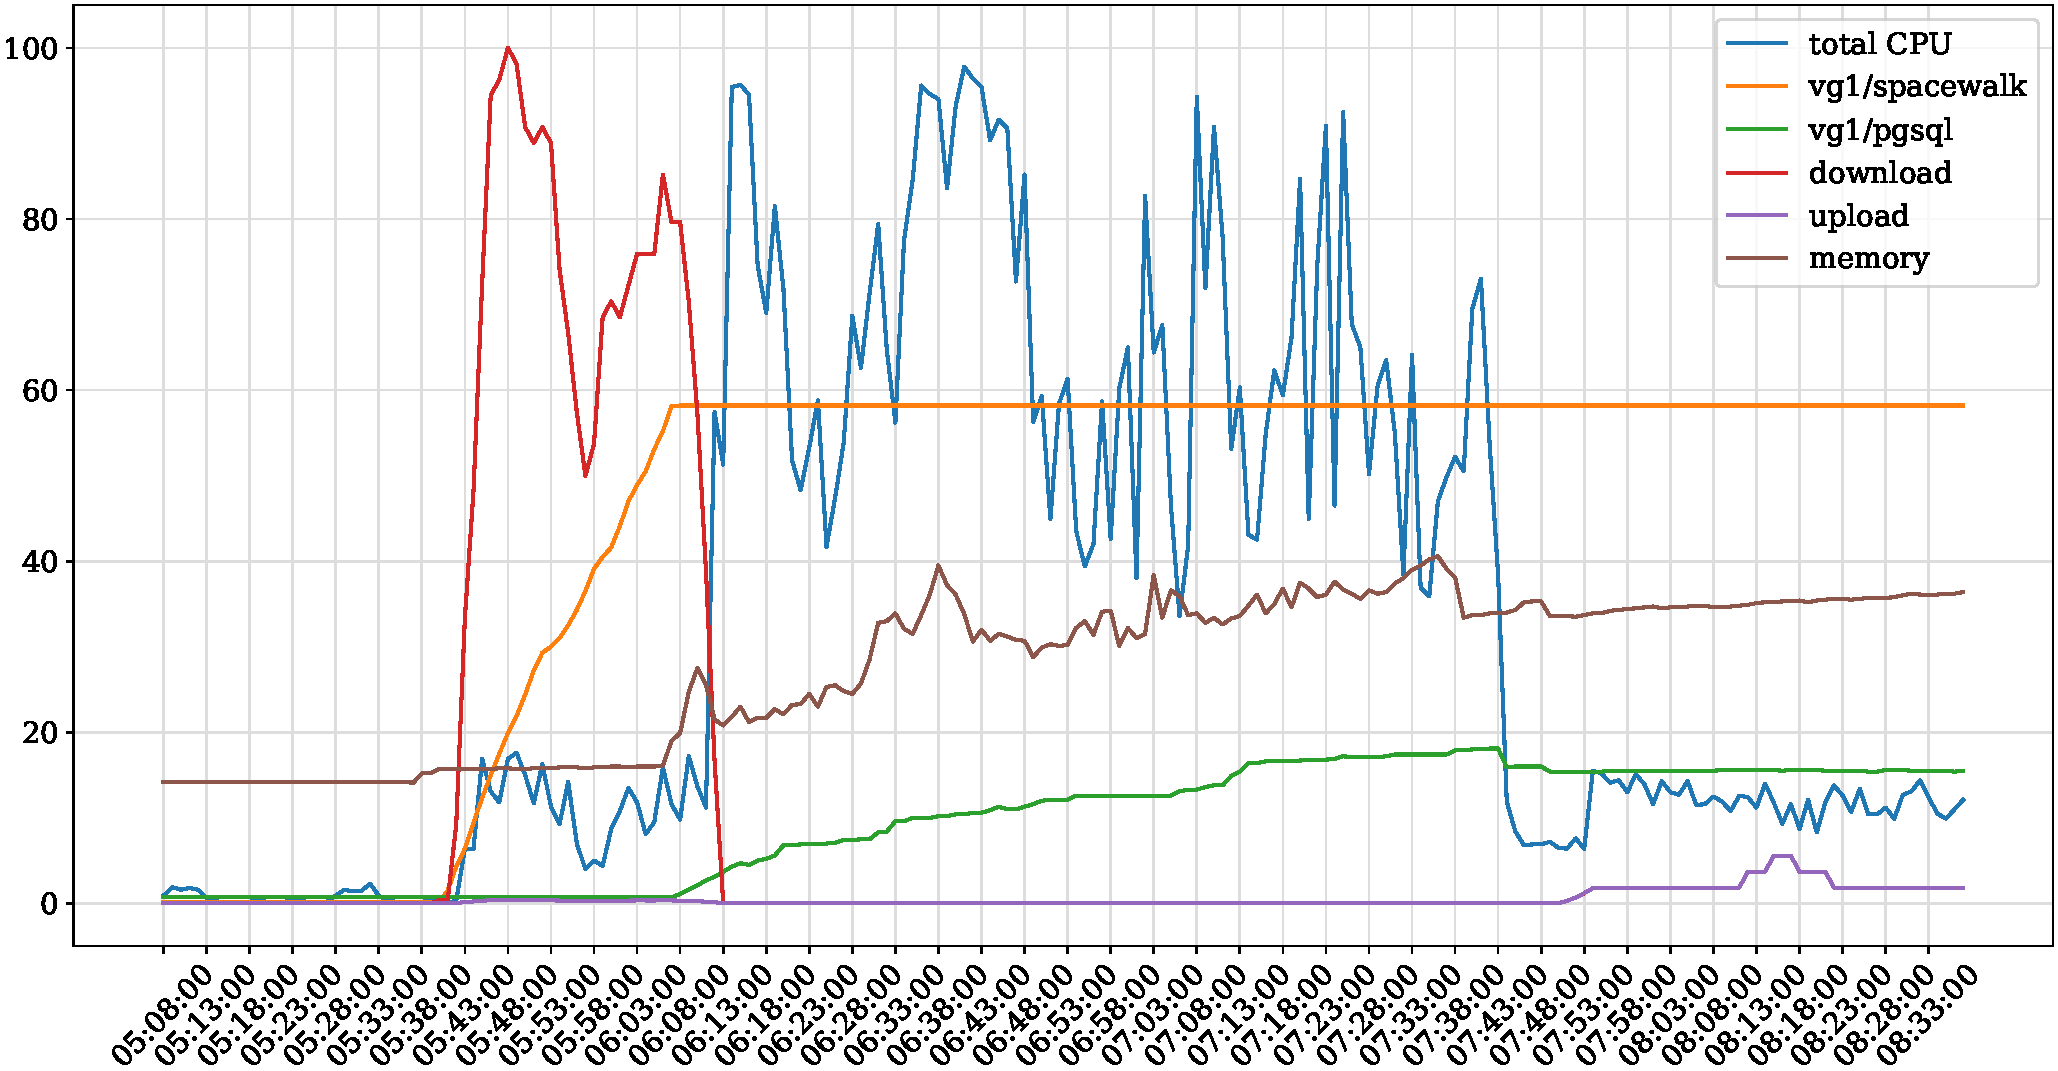
\includegraphics[width=15cm]{figures/reposync-leap-oss-grid.pdf}
	\caption{Az Uyunit futtató virtuális gép terheltsége az egyik telepítőforrás tükrözése során.}
	\label{fig:reposync-chart}
\end{figure}

Egy másik, rövidebb szinkronizálás során a virtuális gépeket futtató gazdagépen figyeltem meg a mérőszámok változását. Ennek érdekessége, hogy így lehetőségem nyílt a processzormagok hőmérsékletének nyomon követésére is. Ezáltal megfigyelhetjük a szervergép hűtésének hatékonyságát: míg a~\acrshort{cpu} kihasználtsága körülbelül 50\%-kal~nőtt, a processzor hőmérséklete csupán 8°C-kal változott, ami körülbelül 20\%-os~növekedést jelent. \Aref{fig:reposync-vhost-cputemp}.~ábráról leolvasható, hogy a processzor-hőmérséklet a~\acrshort{cpu} kihasználtságával összhangban változik, azonban érdemes megjegyezni, hogy a hőmérsékletet megjelenítéséhez egy másik skálát alkalmaztam, így a hőmérséklet-növekedés mértéke arányaiban valóban elmarad a processzorkihasználtság változásától. Az ábrán látható 60\%~körüli \acrshort{cpu}-kihasználtság egyébként közel teljes processzorkihasználtságot jelent a virtuális gépen, ugyanis ez körülbelül 14 mag teljes kihasználtságát jelenti (mivel $ 24 * 0.6  = 14,4 $), azaz a két tétlen~\acrshort{vm} mellett feltehetően az adatbázis-indexelést végző Uyunit futtató virtuális gép kihasználja a rendelkezésére álló 12~magot.

\begin{figure}[ht]
	\centering
	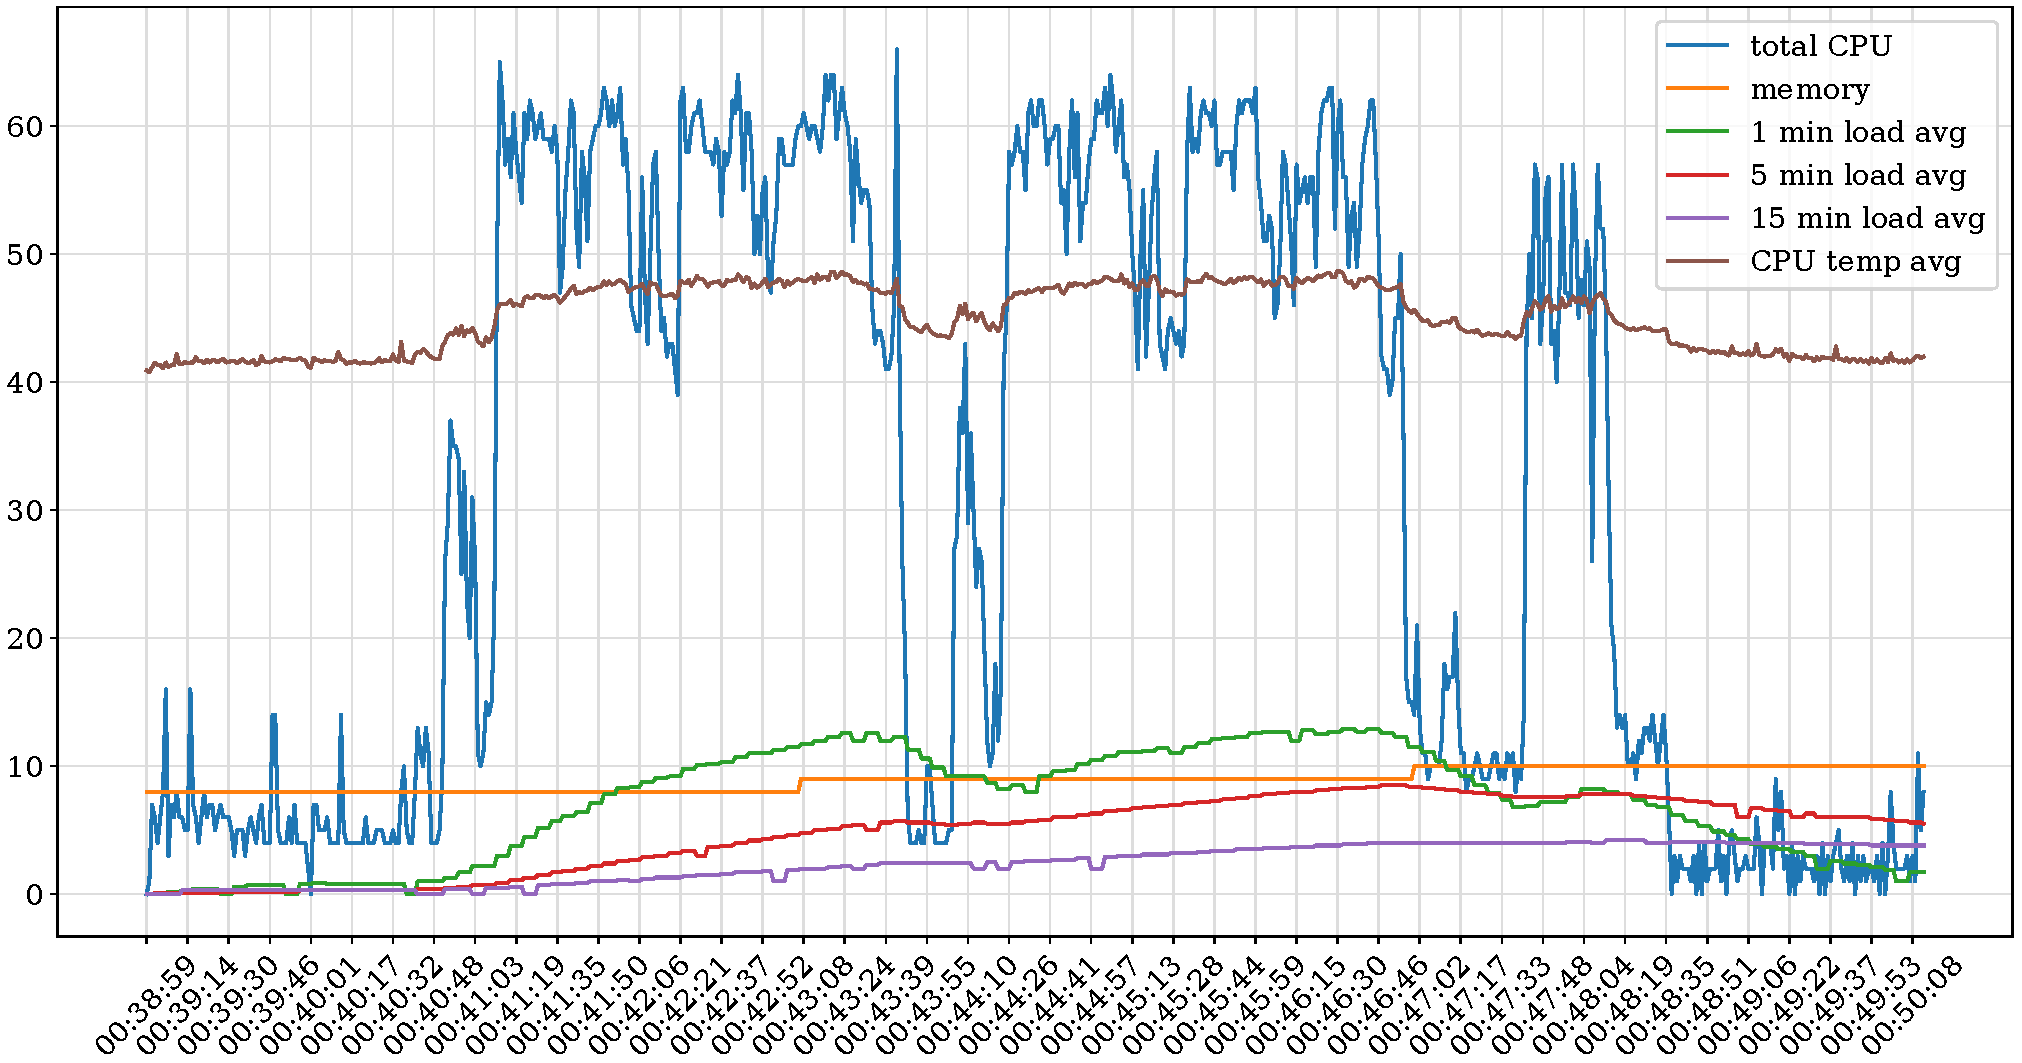
\includegraphics[width=15cm]{figures/reposync-vhost-cputemp.pdf}
	\caption{Processzormagok átlagos hőmérséklete a rendszer terheltsége mellett.}
	\label{fig:reposync-vhost-cputemp}
\end{figure}

\section{Frissítési értesítések}
Teljes körű infrastruktúramenedzsment-megoldásként az Uyuni lehetőséget biztosít a kezelt gépekre telepített csomagok állapotának folyamatos követésére: minden nap, egy előre meghatározott időpontban frissíti a telepítési források adatait, és összeveti az ezekben elérhető szoftververziókat a kezelt gépekre telepítettekével. Ennek köszönhetően a tesztkörnyezet gépeihez  frissítésekről folyamatosan értesültem e-mailben, így mindig naprakész információk álltak a rendelkezésemre a frissítéseket illetően.

Ezek közül kiemelt fontosságúak lehetnek a biztonsági frissítések, hiszen ezek között olyan sérülékenységek javításai is szerepelhetnek, mely kockázatot jelent a rendszer helyes működésére nézve. Ilyen értesítésből körülbelül két és fél hét alatt 9 érkezett, ezeken felül pedig nagyságrendileg 40~további, alacsonyabb prioritású frissítésről kaptam értesítést. Ezen felül az Uyuni felületére belépve az áttekintés oldalon és a rendszerek listájában is látható a kezelt rendszereink frissítéseinek állapota~(\ref{fig:uyuni-security-status}.~ábra).

\begin{figure}[ht]
	\centering
	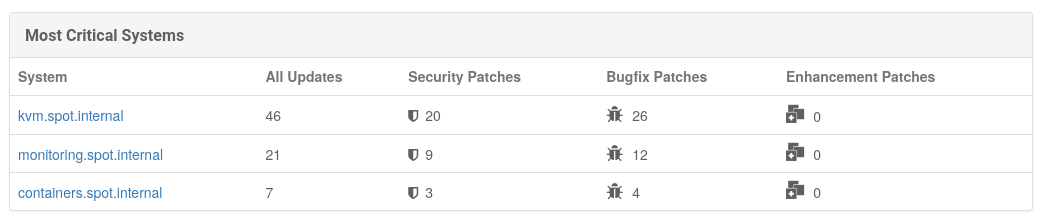
\includegraphics[width=15cm]{figures/uyuni-security-status.png}
	\caption{A kezdőlapon tájékozódhatunk a kliensek biztonsági állapotáról.}
	\label{fig:uyuni-security-status}
\end{figure}